%\modeCorrection

%%%% Définition En-tête et pied de page 
\pagestyle{fancy}
\renewcommand\footrulewidth{1pt}
\fancyhead[L]{Devoir commun de Physique-Chimie}
\fancyhead[R]{Lycée Parc de Vilgénis}
\fancyfoot[C]{\textbf{Page \thepage/\pageref{LastPage}}}

\renewcommand{\thesubsection}{\textcolor{red}{\Roman{section}.\arabic{subsection}}}
\renewcommand{\thesubsubsection}{\textcolor{red}{\Roman{section}.\arabic{subsection}.\alph{subsubsection}}}
\renewcommand{\titreDocu}[1]{
  \refstepcounter{document} % update counter
  \textbf{Exercice \arabic{document} -- #1} 
  \addcontentsline{toc}{document}{\protect\numberline{} #1} % update table of content
}


\renewcommand{\numeroQuestion}{
  \refstepcounter{exercice}
  \vspace*{2pt}
  \hspace{15pt}
  \textcolor{black}{%couleurPrincipale!75!black}{
    \textbf{Q.\arabic{exercice}}
  }
}

\setcounter{section}{0}
\setcounter{document}{0}


%\nomPrenomClasse
\vspace{1cm}

\begin{center}
\begin{Huge}
    DEVOIR COMMUN
\end{Huge}
\end{center}
\vspace{1cm}

\begin{center}
\begin{Huge}
    \'{E}preuve commune de tronc commun
\end{Huge}
\end{center}
\vspace{1cm}

\begin{center}
    \begin{large}
        Jeudi 21 Décembre 2023
    \end{large}
\end{center}

\vspace{2cm}

\begin{center}
    \begin{Large}
        \textbf{PHYSIQUE-CHIMIE}\\
    \end{Large}
\end{center}
\vspace{2cm}


\begin{center}
    \begin{large}
        Durée de l'épreuve : \textbf{2 heures}\\
    \end{large}
\end{center}
\vspace{1cm}
\begin{center}
    \begin{large}
        \textit{L'usage de la calculatrice est autorisé.}\\
    \end{large}
\end{center}
\vspace{1cm}
\begin{center}
    \begin{large}
        Dès que ce sujet vous est remis, assurez-vous qu’il est complet.\\
        Ce sujet comporte \pageref{LastPage} pages numérotées de \thepage/\pageref{LastPage} à \pageref{LastPage}/\pageref{LastPage}.
    \end{large}
\end{center}

\begin{tcolorbox}[colback=red!5!white,colframe=red!75!black,title=\textbf{Consignes : }]
   \begin{enumerate}
       \item Pour les élèves bénéficiant d'un tiers-temps, vous ne traiterez pas les questions : 
       \item Lisez-bien l'énoncé des exercices. Les questions sont pour la plupart indépendantes. Si vous bloquez sur une question, passez à la suivante,
       \item N'oubliez pas d'encadrer/souligner vos résultats.
   \end{enumerate}
\end{tcolorbox}
\newpage

%\begin{tableauCompetences}
%    APP & S'approprier les informations d'un document & & & & \\
%    \hline
%    REA & Utiliser les pourcentages et les fractions  & & & & \\
%     \hline 
%    ANA &  Exploiter les informations extraites des données & & & & \\
%    \hline
%    VAL & Valider/critiquer un modèle & & & &
%\end{tableauCompetences}



\begin{doc}{Le gaz de ville \begin{large}
    / points
\end{large}}
\begin{wrapfigure}{r}{0.3\textwidth}
\vspace{-0cm}
    \centering
      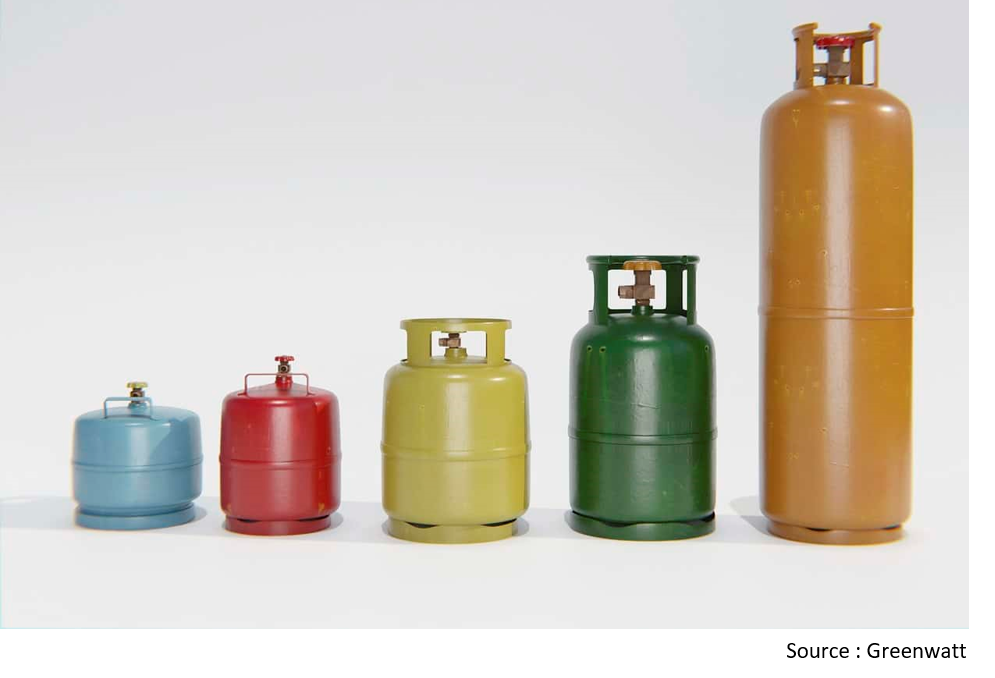
\includegraphics[scale=0.3]{Images/DS/Devoir_Commun/Bouteille_gaz.png}
  \end{wrapfigure}
L'odeur de gaz vous est désagréable, mais c'est pour votre bien ! Le savez-vous ?\\
Le gaz de ville, celui qui arrive dans les habitations par des tuyaux de distribution collective, est principalement constitué de méthane. Le méthane est incolore et inodore, mais alors d'où vient l'odeur si caractéristique du gaz de ville ?\\
Ce que l'on appelle « odeur de gaz » est en réalité dû à un additif ajouté, le TétraHydroThiophène (THT), pour rendre les fuites de gaz détectables et prévenir du danger qu’elles représentent. En effet, le méthane devient fortement explosif lorsqu'il atteint une certaine concentration dans l'air.\\

On considère une bouteille de gaz de ville de volume V=100L. L’étiquette sur la bouteille indique le pourcentage volumique de deux espèces chimiques présentes dans ce mélange :

\begin{center}
    \begin{tabular}{|C{0.45}|C{0.45}|}
        \hline
        \multicolumn{2}{|c|}{\cellcolor{blue!25}Composition du mélange de gaz contenu dans la bouteille} \\
        \hline
        \cellcolor{orange!25}Nom de la substance & \cellcolor{orange!25}Pourcentage volumique \\
        \hline
        TétraHydroThiophène (THT) & 0,10225 \% \\
        \hline 
         Méthane & 99,89775 \%  \\
         \hline
    \end{tabular}
\end{center}
Voici quelques données sur le méthane et le THT :
\begin{center}
    \begin{tabular}{|c|C{0.3}|}
        \hline
        \cellcolor{orange!25}Pictogrammes de sécurité du méthane & \vspace{0.01cm}
            
\includegraphics[scale=0.4]{Images/DS/Devoir_Commun/Picto.png}
         \\
        \hline
        \cellcolor{orange!25}Température de fusion (en $\degreCelsius$) à la pression atmosphérique & $-182,47$ \\
        \hline
        \cellcolor{orange!25}Température de fusion (en $\degreCelsius$) à la pression atmosphérique & $-161,52$ \\
        \hline 
        \cellcolor{orange!25}Masse volumique du méthane (en g.L$^{-1}$) & 0,657 \\
         \hline
    \end{tabular}
\end{center}


\question{Rappeler la définition d’un mélange et proposer un exemple à partir de vos connaissances.}{~}{0}
%\\
\question{Il est conseillé de ne pas conserver une bouteille de méthane à proximité d’une fenêtre exposée au soleil. Justifier à l’aide des pictogrammes de sécurité du méthane.
}{}{0}
%\\
\question{Indiquer l’état physique du méthane à température ambiante (20°C) et à la pression atmosphérique. Justifier}{}{0}
%\\
\question{\`{A} l’aide des documents, déterminer le volume de chaque espèce chimique présente dans la bouteille de gaz de ville.}{~}{0}
%\\
Voici un graphe donnant la masse volumique du mélange méthane/THT en fonction du pourcentage volumique du THT dans le mélange : 
\begin{center}
    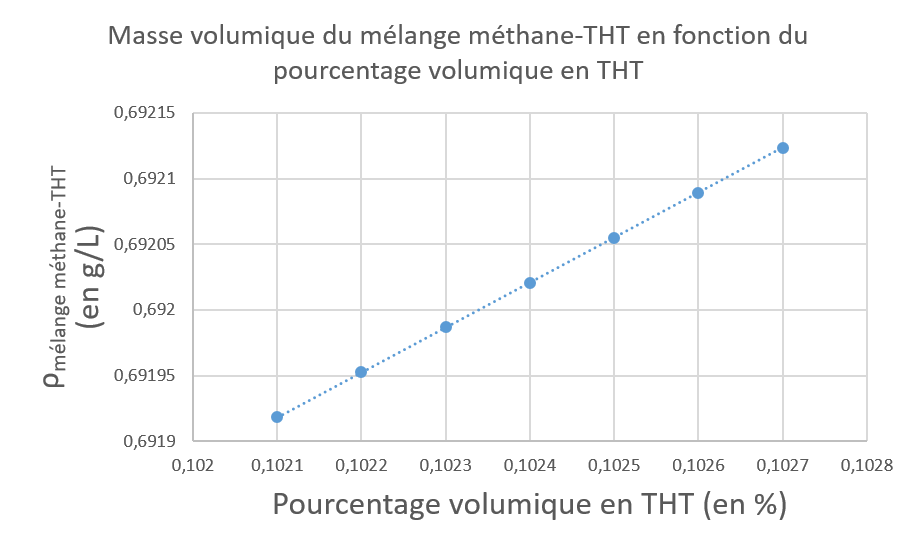
\includegraphics[scale=1]{Images/DS/Devoir_Commun/Graphe_rhovspourcentagevol.png}
\end{center}
\question{Déterminer graphiquement la masse volumique du mélange dans la bouteille de gaz de ville. Vous ferez apparaître la construction sur le graphique.}{~}{0}
%\\
\textbf{Pour la question suivante, toute tentative de réponse même non aboutie sera valorisée.}\\
\question{La norme imposée au gaz de ville est qu’il doit contenir entre $15\times10^{-1}$~mg et $40\times10^{-1}$~mg de THT par litre de gaz. La masse de THT présente dans la bouteille de gaz étudiée respecte-t-elle la norme imposée au gaz de ville ? Justifier en rédigeant une réponse scientifiquement argumentée.}{La masse volumique de l'eau est $\rho_{eau}=1000$~kg.m$^{-3}$.}{0}
%\\
\end{doc}

%%%%%%%%%%%%%%%%%%%%%%%%%%%%%%%%%
\newpage
%%%%%%%%%%%%%%%%%%%%%%%%%%%%%%%%%

\begin{doc}{Solutions aqueuses \begin{Large}
    /points
\end{Large}}
\begin{wrapfigure}{r}{0.3\textwidth}
\vspace{-1cm}
    \centering
      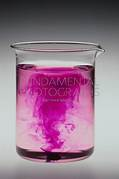
\includegraphics[scale=1.0]{Images/DS/Devoir_Commun/Permanganate.png}
  \end{wrapfigure}
\og Le permanganate de potassium est un solide gris-violet de formule \chemform{KMnO_4}. Dissous dans l’eau, il donne des solutions de couleur violette.\\
Pour soigner les érythèmes (irritations de la peau), il est recommandé d’utiliser des solutions aqueuses de permanganate de potassium de concentration en masse égale à $0,10$~g$\cdot$L$^{-1}$.\\
En solution aqueuse à $0,50$~g$\cdot$L$^{-1}$, le permanganate de potassium est également utilisé comme désinfectant pour laver les légumes dans les pays tropicaux.\fg
\begin{flushright}
    \textit{D’après le site \url{ societechimiquedefrance.fr/permanganate-de-potassium}}.
\end{flushright}

L’objectif de l’exercice est d’estimer la concentration d’une solution aqueuse S de permanganate de potassium afin de valider ou non son utilisation pour soigner les érythèmes ou pour laver les légumes.\\

Pour cela, on prépare 250 mL d’une solution aqueuse $S_0$ de permanganate de potassium de concentration en masse $C_{m,0} = 0,60$~g$\cdot$L$^{-1}$ par dissolution dans l’eau d’une masse appropriée de permanganate de potassium solide.\\


\question{Identifier le solvant et le soluté des solutions utilisées pour soigner les érythèmes ou pour laver les légumes.}{Solvant : eau, soluté : \chemform{KMnO_4}.}{0}
%\\
\question{Donner le nom de la technique utilisée pour préparer la solution $S_0$.}{Il s'agit d'une dissolution.}{0}
%\\
\question{Donner l’expression de la concentration en masse $C_m$ d’une solution en fonction de la masse de soluté $m_{\text{soluté}}$ et du volume de solution $V_{\text{solution}}$.}{}{0}
%\\
\question{En déduire la valeur de la masse de permanganate de potassium qui a été dissoute pour préparer 250 mL de solution $S_0$.}{~}{0}
%\\
On prépare ensuite cinq solutions $S_1$, $S_2$, $S_3$, $S_4$ et $S_5$ en prélevant différents volumes de solution aqueuse $S_0$ de permanganate de potassium de concentration en masse $C_{m,0} = 0,60$~g$\cdot$L$^{-1}$ et en y ajoutant de l’eau distillée pour obtenir un volume de 50,0 mL (voir tableau ci-dessous).
\begin{center}
    \begin{tabular}{|C{0.1}|C{0.2}|C{0.2}|C{0.2}|}
        \hline
        \cellcolor{blue!25}Solution & \cellcolor{blue!25}Volume de solution $S_0$ à prélever (mL) & \cellcolor{blue!25}Volume de solution obtenu (mL) & \cellcolor{blue!25}Concentration en masse de la solution (g$\cdot$L$^{-1}$) \\
        \hline 
        $S_1$ & 2 & 50,0 & 0,024 \\
        \hline
        $S_2$ & 5 & 50,0 & 0,060 \\
        \hline
        $S_3$ & 10 & 50,0 & 0,12 \\
        \hline
        $S_4$ & 15 & 50,0 & 0,18 \\
        \hline
        $S_5$ & ~? & 50,0 & 0,24 \\
        \hline
    \end{tabular}
\end{center}

\question{Donner le nom de la technique utilisée pour préparer les cinq solutions $S_1$, $S_2$, $S_3$, $S_4$ et $S_5$.}{Il s'agit d'une dilution.}{0}
%\\
\question{Écrire le protocole expérimental qui a été suivi pour préparer 50,0 mL de solution $S_1$. Préciser soigneusement le nom du matériel utilisé.}{~}{0}
%\\
\question{Déterminer la valeur du volume de solution S0 qui a été prélevé pour préparer 50,0 mL de solution $S_5$. Justifier précisément le calcul effectué.}{~}{0}
%\\
On verse les cinq solutions $S_1$, $S_2$, $S_3$, $S_4$ et $S_5$ dans des tubes à essais : on obtient ainsi une échelle de teintes (voir photo ci-dessous).
\begin{center}
    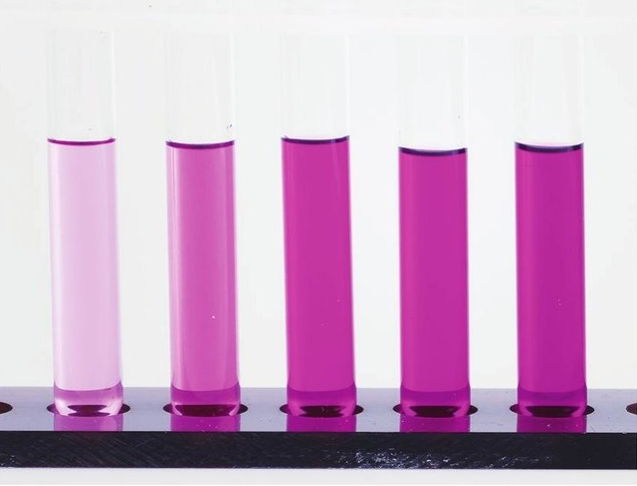
\includegraphics[scale=0.5]{Images/DS/Devoir_Commun/Echelle_teinte.png}
\end{center}
On verse ensuite la solution S dans un sixième tube à essais. On constate que la teinte de la solution S est comprise entre celles des solutions $S_2$ et $S_3$.\\
\question{Déterminer un encadrement de la concentration en masse de la solution S}{$0,060~\text{g$\cdot$L$^{-1}$}<C_{m,0}<0,12~\text{g$\cdot$L$^{-1}$}$}{0}
%\\
\question{En déduire si la solution $S$ peut être utilisée pour soigner les érythèmes ou pour laver les légumes.}{~}{0}
\end{doc}

\begin{doc}{Le son d’une guitare
 \begin{Large}
    / points
\end{Large}}
Une guitare se compose d'un coffre auquel est accroché un manche sur lequel sont tendues des cordes métalliques ou en nylon. La photo ci-dessous présente une guitare ainsi qu'un zoom sur une partie du manche après avoir frotté les cordes :

\begin{center}
    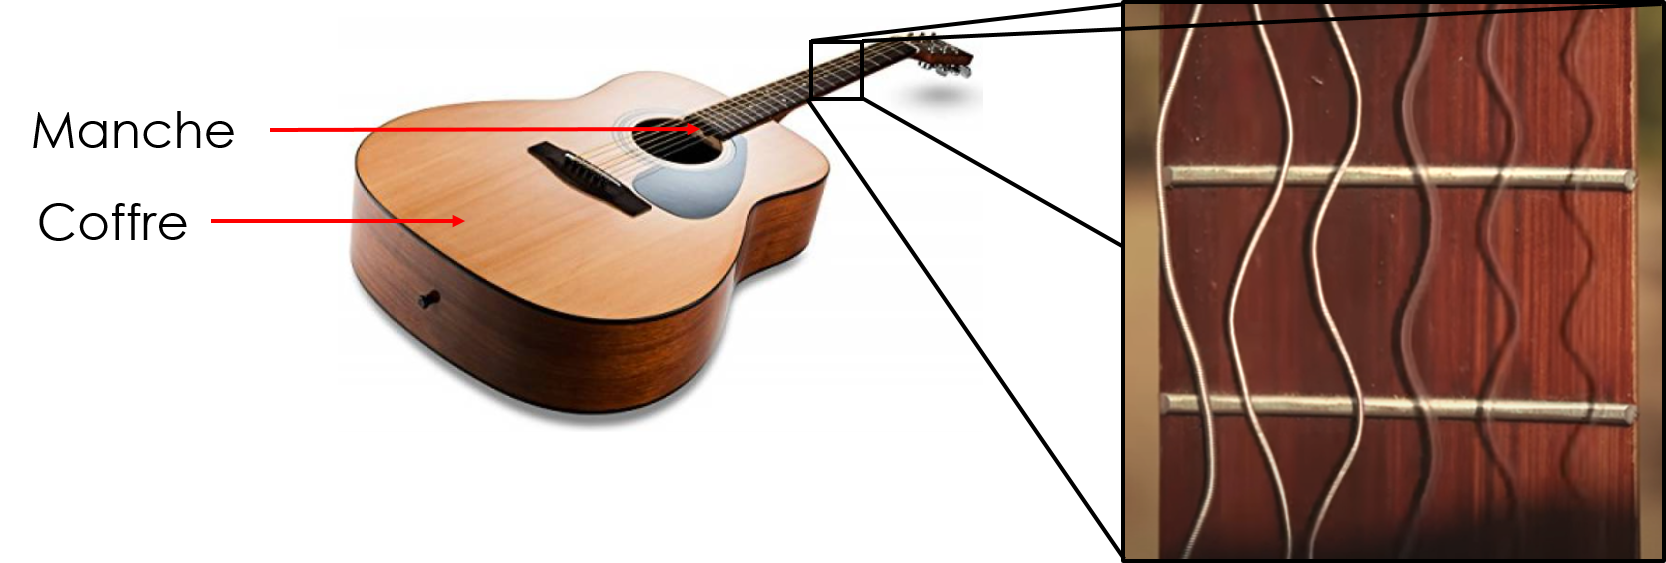
\includegraphics[scale=0.5]{Images/DS/Devoir_Commun/Guitare.png}
\end{center}

Voici un tableau des notes (do, ré, mi, fa, sol, la, si) et des fréquences (en Hz) correspondantes de la gamme tempérée :
\begin{center}
    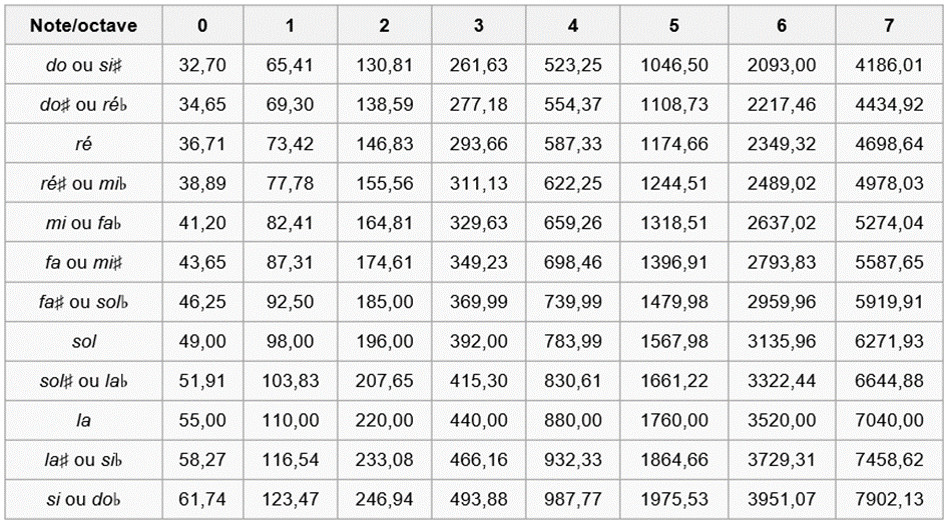
\includegraphics[scale=0.7]{Images/DS/Devoir_Commun/Notes_guitare.png}
\end{center}
De la plus épaisse à la plus fine, les notes correspondant aux cordes de la guitare, jouées \og à vide \fg~, c’est-à-dire en les laissant sonner librement sur toute leur longueur, sont  \og mi2, la2, ré3, sol3, si3, mi4 \fg~.

\question{Rappeler l’origine du son émis par une guitare.}{Les cordes vibrent et font vibrer les molécules d'air de proche en proche.}{0}
%\\
\question{Donner l'intérêt physique du coffre de la guitare.}{Le coffre sert de caisse de résonance, c'est-à-dire qu'il sélectionne et amplifie et le son émis par le frottement des cordes de guitare.}{0}
%\\
\question{Rappeler la condition pour que le son se propage dans un milieu. Donner ce milieu et rappeler la vitesse de propagation du son dans ce milieu.}{Il faut un milieu matériel pour que le son puisse se propager. Ici, le milieu est l'air et la vitesse vaut (à $15\degreCelsius$) 340~m$\cdot$s$^{-1}$.}{0}
%\\
\question{Si l’auditeur se trouve à une distance d=1km, calculer la durée $\Delta t$ que met le son à se propager jusqu’à l’auditeur. \textit{(Bonus) : l'auditeur parviendre-t'il a entendre ce son ? Justifier.}}{~}{0}
%\\
\question{Rappeler le domaine des fréquences audibles pour un être humain.}{Entre 20~Hz et 20000~Hz.}{0}
%\\
\question{Un chat est capable d’entendre des fréquences comprises entre 20 Hz et 60 kHz. Pourrait-il entendre la note la plus grave jouée avec une guitare ? Justifier la réponse.}{Oui car la note la plus grave sonne à la fréquence 32,70~Hz qui est comprise dans le domaine de fréquence audible du chat.}{0}
%\\
\question{Donner les fréquences des 6 cordes jouées à vides à la guitare.}{~}{0}
%\\
\question{Entre la première corde de mi et la dernière corde de mi, donner le son le plus aigu. Justifier votre réponse en vous appuyant sur les fréquences respectives de ces 2 notes.}{~}{0}
%\\
Un ingénieur du son a enregistré une note émise par une guitare, à l’aide d’un microphone relié à un système informatisé. Voici le signal enregistré :
\begin{center}
    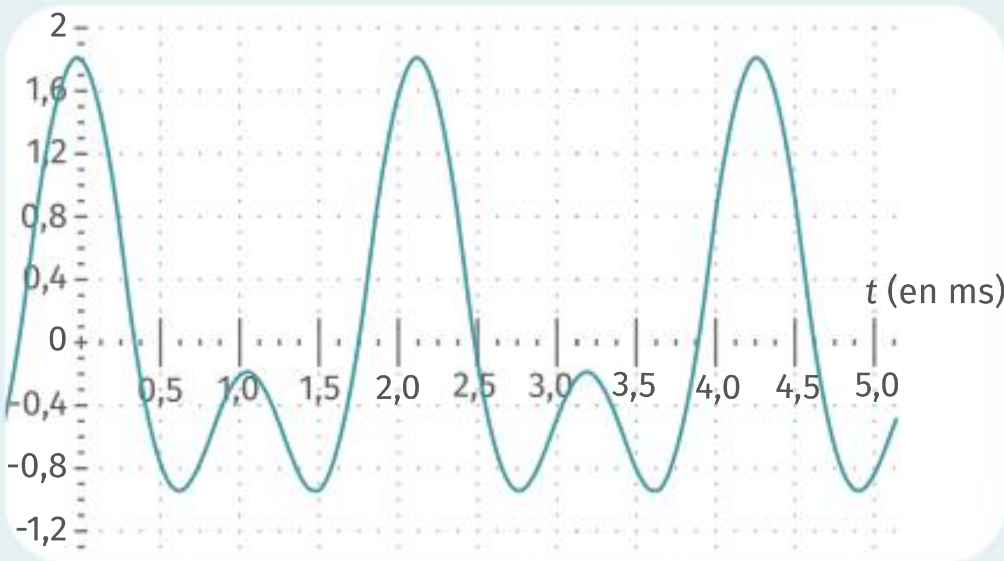
\includegraphics[scale=0.5]{Images/DS/Devoir_Commun/Signal_guitare.PNG}
\end{center}
\question{Rappeler le lien entre la fréquence et la période d’un signal sonore puis déterminer la fréquence $f$ de la note jouée.}{~}{0}

\end{doc}
\vspace{2cm}
\begin{center}
\begin{Huge}
    \textbf{FIN DU SUJET.}
\end{Huge}
\end{center}